\documentclass[]{article}

%%%%%%%%%%%%%%%%%%%
% Packages/Macros %
%%%%%%%%%%%%%%%%%%%
\usepackage{amssymb,latexsym,amsmath}     % Standard packages

\usepackage{graphicx}
\usepackage[colorlinks=true, allcolors=blue]{hyperref}

\usepackage[round,authoryear]{natbib}
\bibliographystyle{plainnat}
\usepackage{bookmark}

\usepackage{tikz}
\usepackage{tocloft}

\usepackage{placeins}

\usepackage{lipsum} % Add this line in the preamble if not already included

%%%%%%%%%%%
% Margins %
%%%%%%%%%%%
\usepackage[margin=0.8in]{geometry}

\title{Sample \LaTeX ~File}
\author{Gosha Syunyaev}

%%%%%%%%%%%%
% Document %
%%%%%%%%%%%%
\begin{document}

\maketitle

\begin{abstract}
  This document represents the output from the file ``example\_latex.tex" once compiled using your favorite \LaTeX compiler.  This file should serve as a good example of the basic structure of a ``.tex" file as well as many of the most basic commands needed for typesetting documents involving mathematical symbols and expressions. 
\end{abstract}

\tableofcontents

\newpage

\section{Introduction}

This document serves as an introduction to using \LaTeX{} for typesetting documents. Examples of commonly used commands and features are listed below to help you get started.

\section{Some examples to get started}

\subsection{How to create Sections and Subsections}

Use the section and subsection commands to organize your document. \LaTeX{} automatically handles the formatting and numbering according to the document class you've chosen.

\subsection{How to include Figures}

To include an image, use the \texttt{includegraphics} command within a figure environment. Add a caption using the \texttt{caption} command. See the code for Figure \ref{fig:frog} for an example.

\FloatBarrier

\begin{figure}[htbp]
\centering
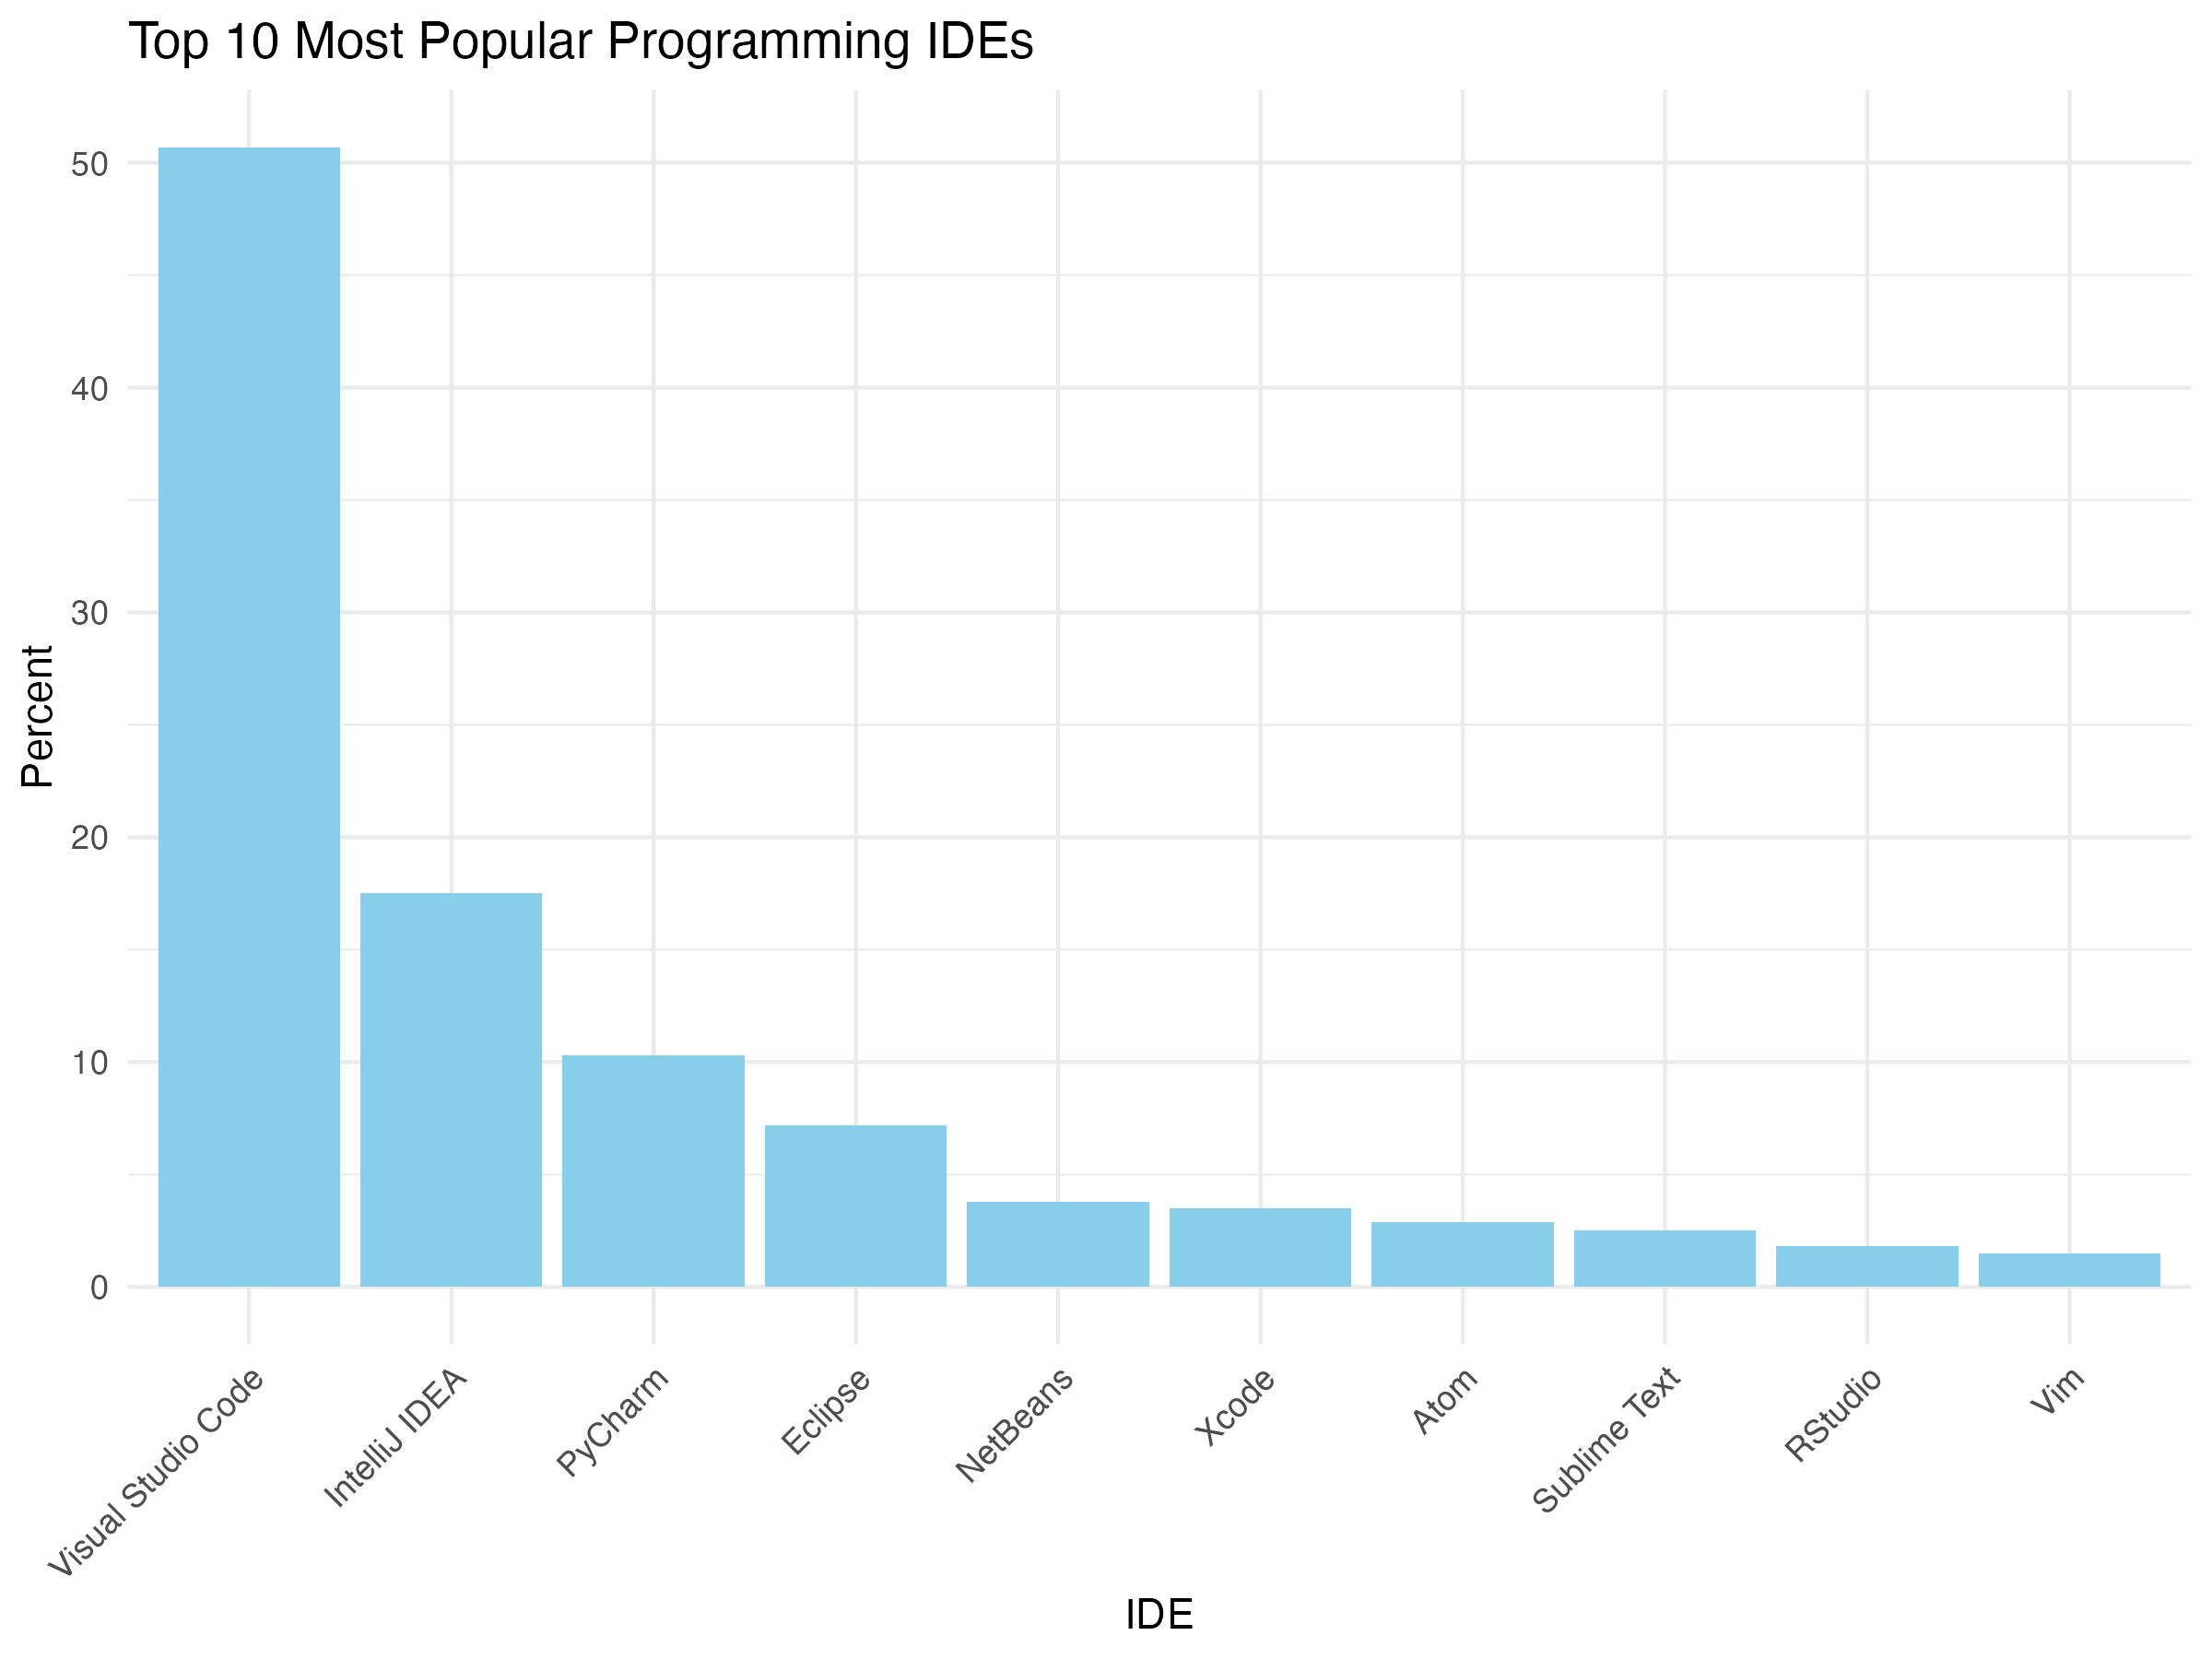
\includegraphics[width=0.6\textwidth]{supp/ide_plot.jpeg}
\caption{\label{fig:frog}This is an example figure.}
\end{figure}

Here is a simple example of a diagram created using TikZ:

\begin{figure}[htbp]
  \centering
  \begin{tikzpicture}
    % Nodes
    \node (C) at (1,2) {C};
    \node (X) at (0,0) {X};
    \node (Y) at (2,0) {Y};
    
    % Arrows
    \draw[->] (C) -- (X) node[midway, left] {+};
    \draw[->] (C) -- (Y) node[midway, right] {-};
    \draw[->] (X) -- (Y) node[midway, below] {-};
  \end{tikzpicture}
\caption{\label{fig:causal}A simple causal diagram.}
\end{figure}


\subsection{How to add Tables}

Use the table and tabular environments for creating tables. See Table~\ref{tab:widgets} for an example.

\begin{table}
\centering
\begin{tabular}{l|r}
Item & Quantity \\\hline
Widgets & 42 \\
Gadgets & 13
\end{tabular}
\caption{\label{tab:widgets}An example table.}
\end{table}

\subsection{How to add Lists}

Create lists with automatic numbering:

\begin{enumerate}
  \item First item,
  \item Second item.
\end{enumerate}
\dots or bullet points:
\begin{itemize}
  \item First bullet,
  \item Second bullet.
\end{itemize}

\subsection{How to write Mathematics}

\LaTeX{} excels at typesetting mathematics. Let $X_1, X_2, \ldots, X_n$ be a sequence of independent and identically distributed random variables with $\text{E}[X_i] = \mu$ and $\text{Var}[X_i] = \sigma^2 < \infty$, and let

$$S_n = \frac{X_1 + X_2 + \cdots + X_n}{n} = \frac{1}{n}\sum_{i=1}^{n} X_i$$

denote their mean. Then as $n$ approaches infinity, the random variables $\sqrt{n}(S_n - \mu)$ converge in distribution to a normal $\mathcal{N}(0, \sigma^2)$.

\subsection{How to add Citations and a References List}

Upload a \verb|.bib| file containing your BibTeX entries. Cite entries using the \verb|\cite| command, like this: \cite{greenwade93}. Specify a bibliography style and the filename of the \verb|.bib| file.

\bibliography{supp/sample}

\end{document}